\documentclass{csse4400}

\usepackage{tikz}
\usetikzlibrary{positioning}
\usetikzlibrary{arrows}

\usepackage{float}
\usepackage{enumitem}
\usepackage{languages}
\usepackage{changepage}

\title{yLearn}
\author{Brae Webb \& Richard Thomas}

\date{\week[tutorial]{4}}
\begin{document}

\maketitle

\section{Brief}

Following the overwhelming success of online learning,
the University of Queensland is seeking to expand its online course catalogue.
To do so, they are deploying the online Learning Management System (LMS),
yLearn, an alternative to Blackboard written from the ground up.
You are leading the team at UQ's Information Technology Services (ITS) to design this system.

Blackboard utilised a monolithic architecture.
This quickly became a problem as the system grew in size and complexity.
The system was difficult to maintain and nearly impossible extend.
ITS is looking to avoid this problem going forward
by developing a distributed system that more naturally fits the small team structure while maintaining core shared data.
This will allow the team to maintain the functionality under their care, and eventually,
extend the system with new features such as online examinations.

\section{Requirements}

\begin{enumerate}
\item The system should be a distributed system that is designed to be modular and extensible.
\item The backend should support the core functionality of the LMS, such as managing courses, student enrolment, and grading.
\item The backend should support the integration of new features, such as online examinations, in the future.
\item The backend should be designed to be scalable and fault-tolerant.
\end{enumerate}

\section{Outline}

\subsection*{Introduction (5 minutes)}
Introduction to the brief,
moving from monolithic to distributed systems,
what are the core requirements of the system,
etc.

\subsection*{Design (8 minutes)}
In small groups, discuss potential approaches to designing this system.
You can use any tools you like,
but you should be able to explain your design to the class.
If you are using digital tools,
\link{excalidraw}{https://excalidraw.com/} is useful for sketching.
Your design does not need to be complete nor perfect,
try to be creative so that we can discuss the pros and cons of various design options.


\subsection*{Discussion (7 minutes)}
With the class, present a few of the designs and discuss the pros and cons of each.
Consider the following questions:
\begin{itemize}
\item Which quality attributes are prioritised in this design?
\item Are individual ITS teams able to maintain the features/products that they are responsible for?
\item How would this design scale to support more users?
\item What trade-offs are we making?
\item Imagine that you have to integrate \link{TurnItIn's academic integrity suite}
      {https://www.turnitin.com.au/solutions/higher-education}, which consists of four components.
      Three of these, \link{similarity}{https://www.turnitin.com.au/products/similarity/},
      \link{originality}{https://www.turnitin.com.au/products/originality/},
      and \link{feedback studio}{https://www.turnitin.com.au/products/feedback-studio/}
      are used in managing student assessment submissions.
      With your design, how would you go about doing this?
\item Does the proposed design maintain data consistency
      such that it is not possible for an instructor to see grades different from what students see?
\end{itemize}

\subsection*{Diagram (30 minutes)}
Design a C4 diagram of your proposed system.
Your design sketch should include:
\begin{itemize}
\item A high-level overview of the system, including any architectural patterns used.
\item Which distributed components are included in the initial feature set.
\item How the different distributed components communicate with each other.
\item A brief description of any component interfaces present in the design.
\item A description of how the system handles scaling.
\end{itemize}

%\subsection*{Service Details}
%Assume one of the services is responsible for content management.
%What are some important
%\begin{itemize}
%    \item components that would deliver the service behaviour,
%    \item features accessed via the API, and
%    \item data elements that would need to be stored.
%\end{itemize}
%%Content being held in a tree structure, with nodes being layers in the content or content items.

\subsection*{Challenge 1: User Authentication}
How would you handle user authentication in the system?
Research some standard tactics for authentication.
UQ's Single Sign-On (SSO) uses SAML authentication,
how would you integrate with this protocol?
If UQ wanted to enable self-managed account creation and course enrolment,
how would you integrate with that?

\subsection*{Challenge 2: Fault Tolerance}
With a distributed system,
there is always a risk of server failure or other system errors.
How can you design the system to be fault-tolerant and recover from failures quickly and efficiently?
Are their particular components of your system that would necessitate services to fail?
Could you remove that dependency?
What would you be trading off?

\subsection*{Challenge 3: Ad-hoc Tooling}
Often academics write their own tooling to help operate courses.
Ideally, these academics would not place additional burden on ITS staff by making requests to integrate their own tool with the LMS system.
How would you design a system that allows academics to deploy their own tools based on the permission they already have for their course?
How would this system avoid having to require ITS involvement?
How would this system preserve user data security?


\appendix

\section{Blackboard Architecture}
This a C4 model based loosely on an old version of the Blackboard architecture.
You can use this as a starting point for your yLearn replacement.
The model no longer reflects the current state of the Blackboard architecture.
You can download the model from the \link{course website}{https://csse6400.uqcloud.net/resources/blackboard.zip}.
You can upload it to the \link{Structurizr cloud platform}{https://structurizr.com/} to edit it during the tutorial.

\begin{figure}[h!]
\centering
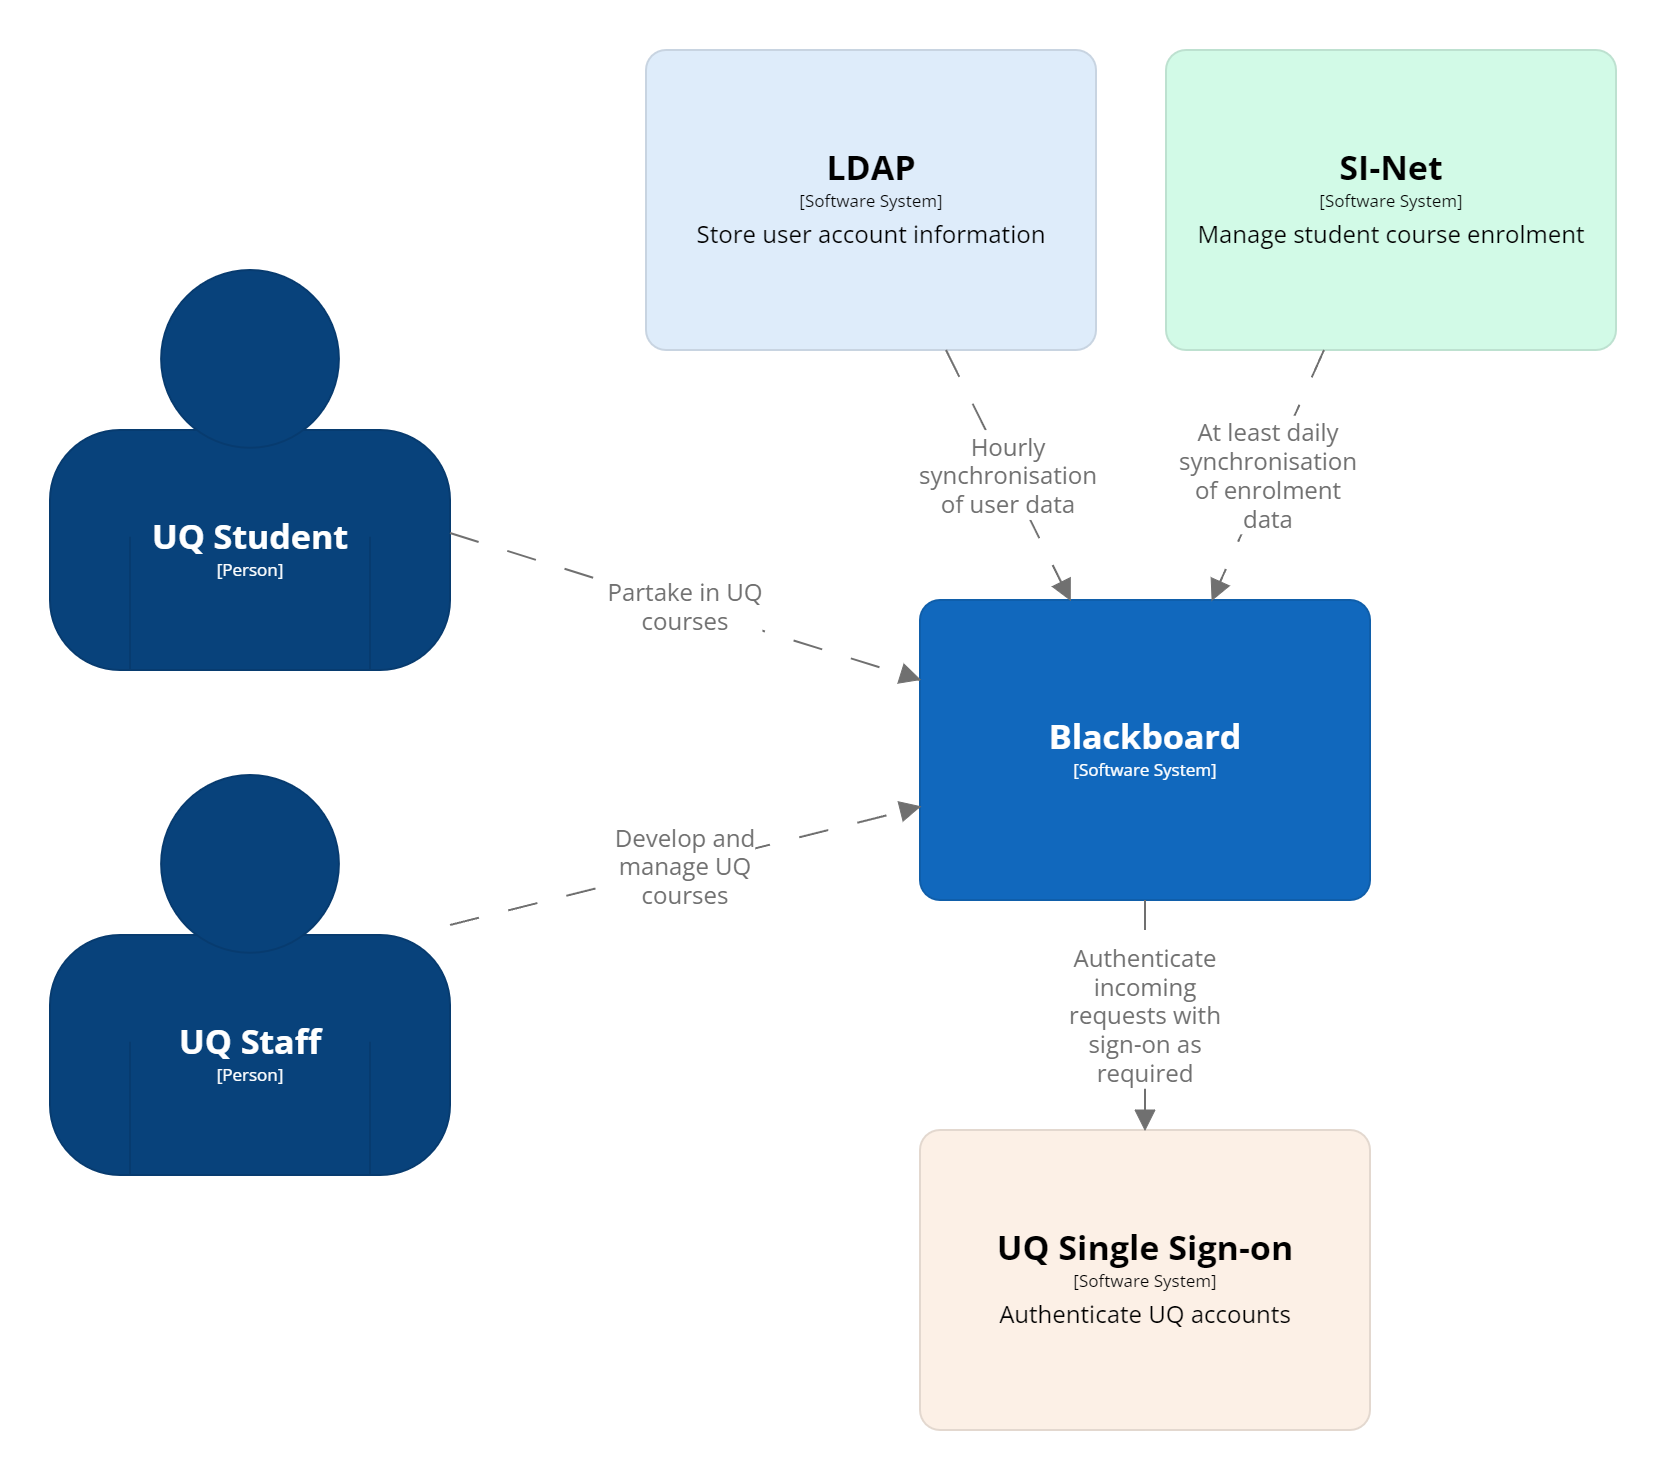
\includegraphics[width=0.9\textwidth]{images/context}
\caption{Blackboard context diagram}
\end{figure}
\vspace{2em}

\begin{figure}
\centering
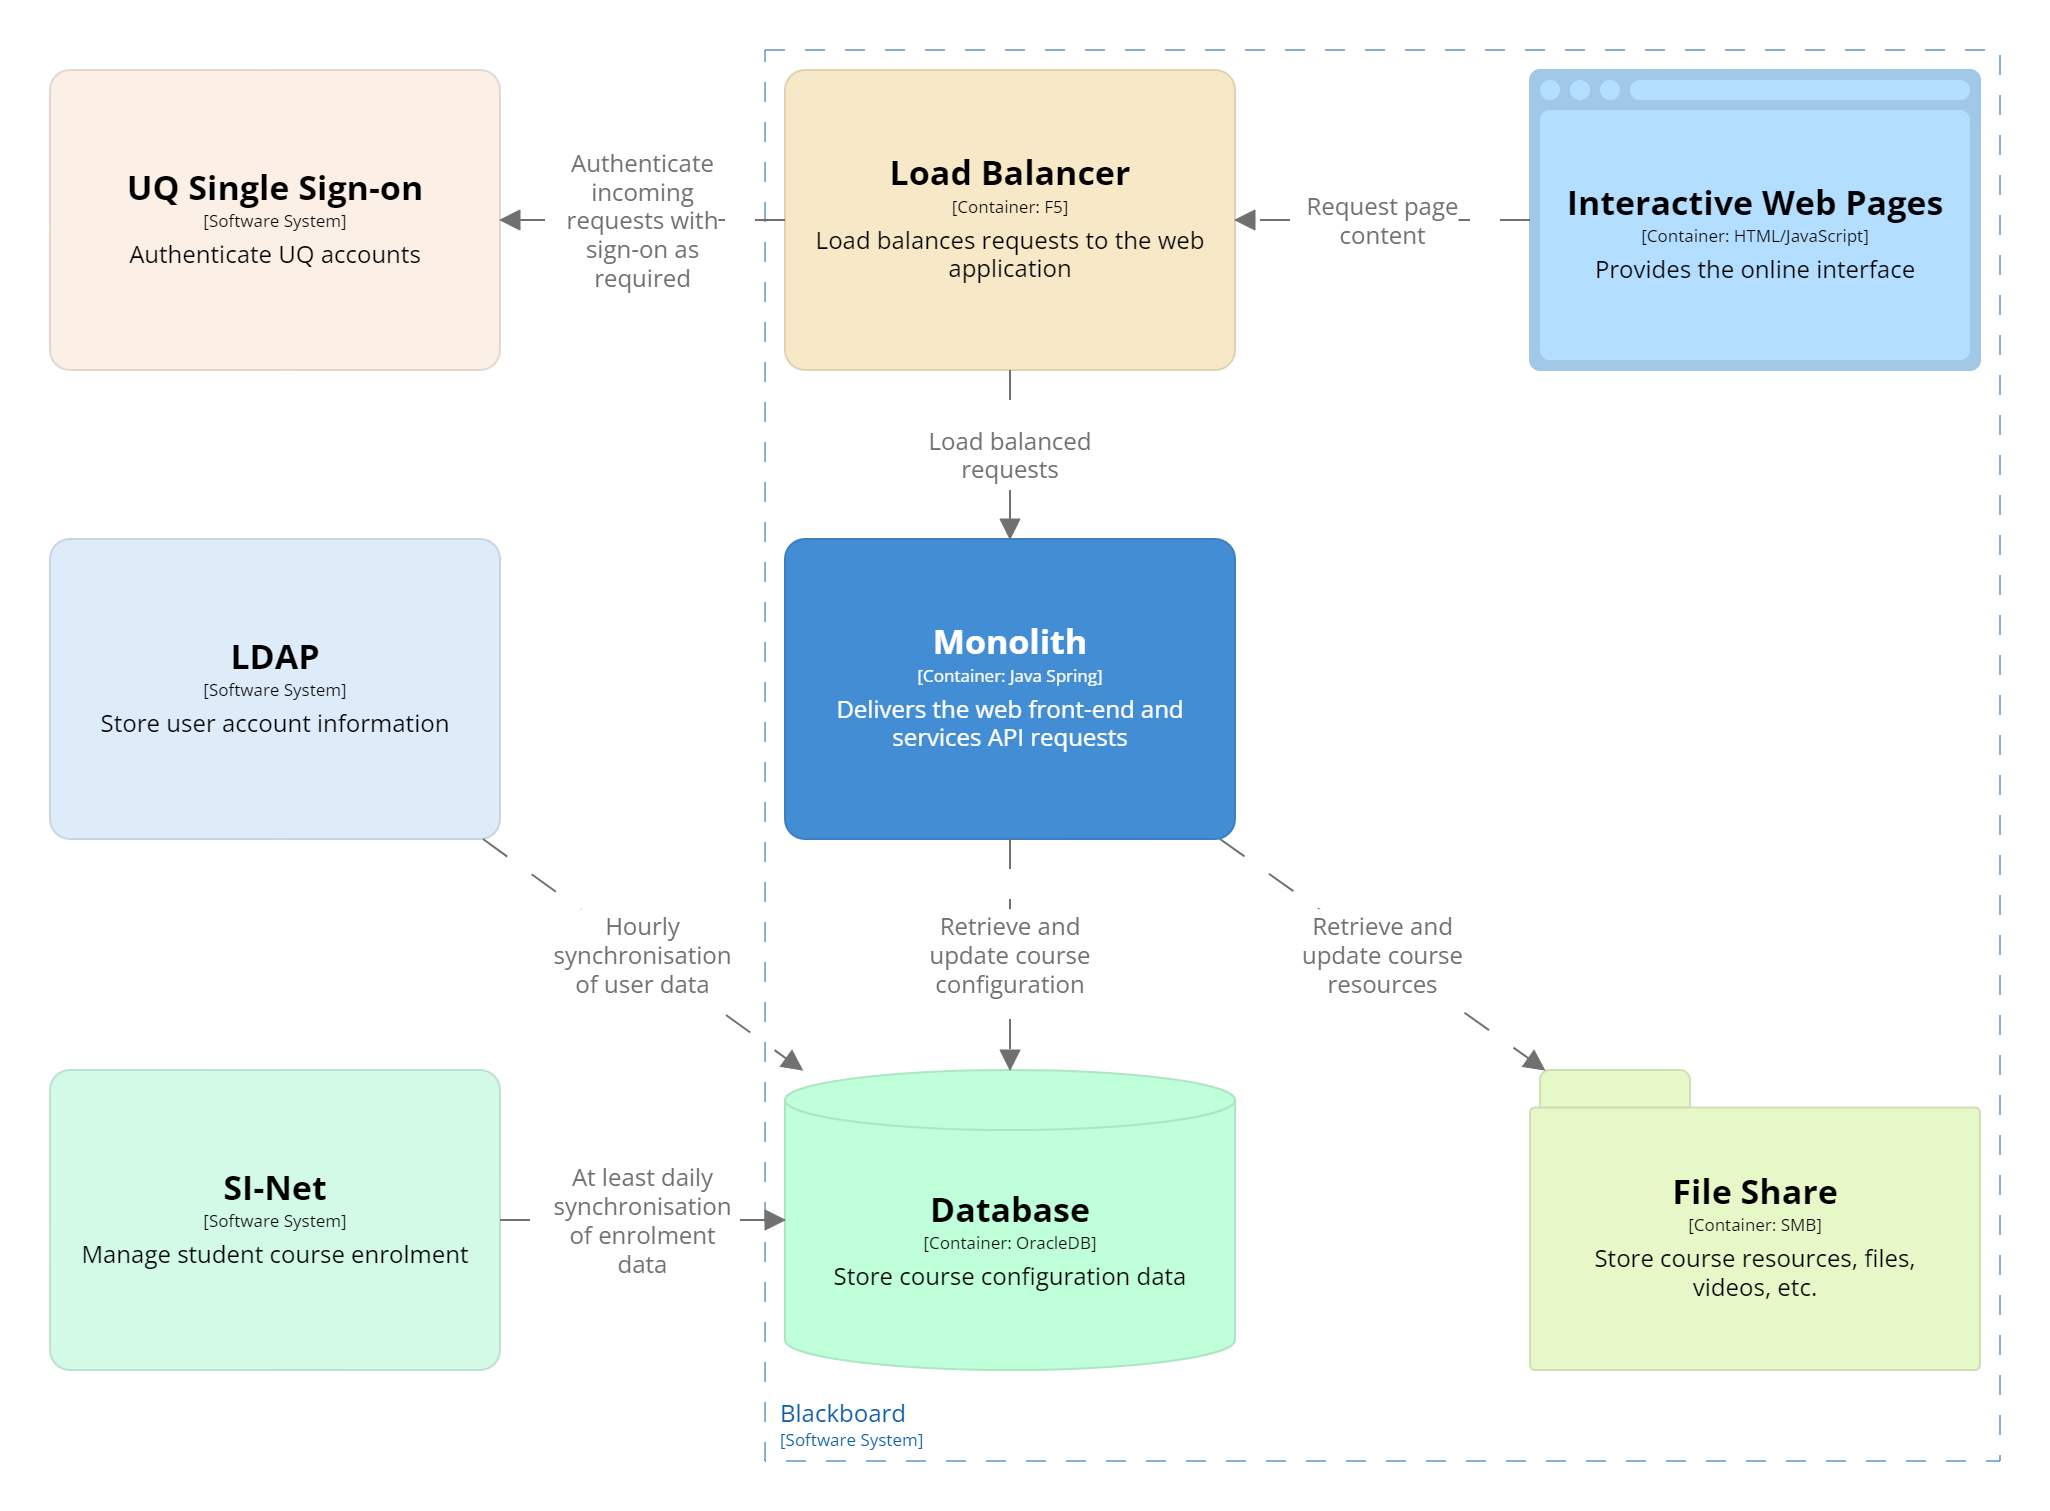
\includegraphics[width=\textwidth]{images/container}
\caption{Blackboard container diagram}
\end{figure}

\begin{figure}
\begin{adjustwidth}{-11mm}{-11mm}
\centering
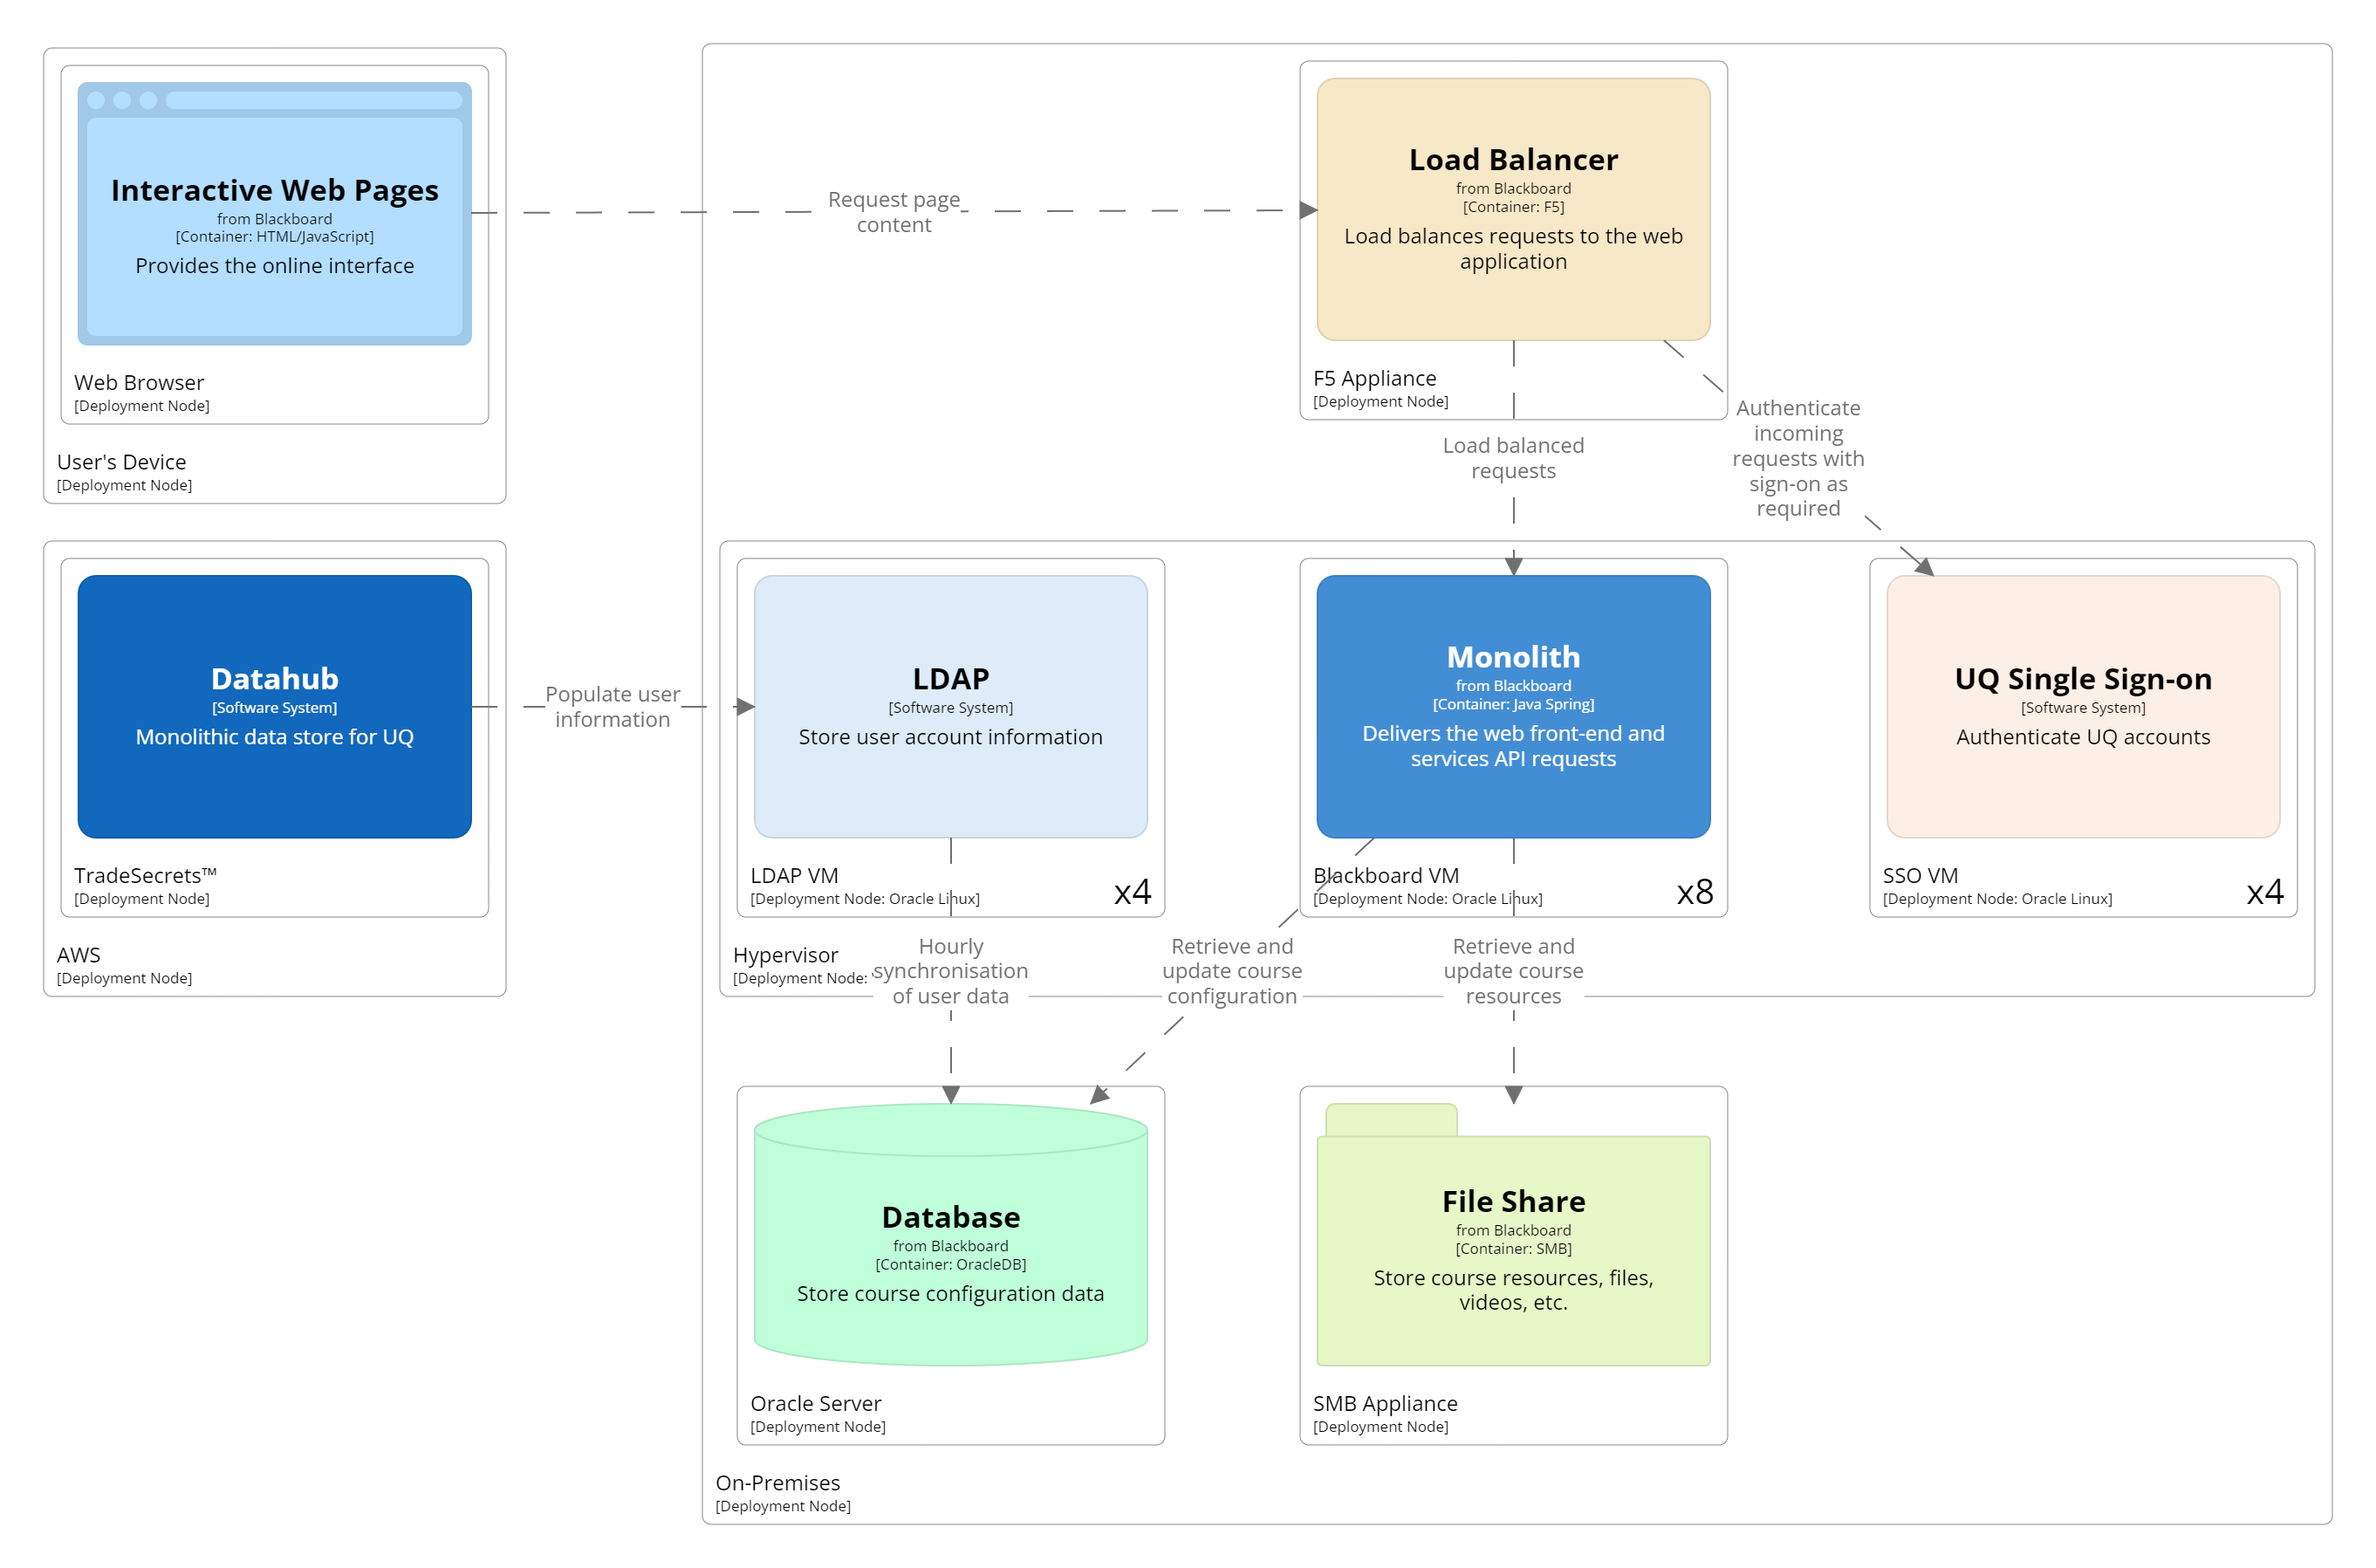
\includegraphics[width=0.98\paperwidth]{images/deployment}
\caption{Blackboard deployment diagram}
\end{adjustwidth}
\end{figure}

\end{document}
